\documentclass[a4paper, 12pt]{article}

\usepackage{hyperref}
\usepackage[warn]{mathtext}
\usepackage[utf8]{inputenc}
\usepackage[T2A]{fontenc}
\usepackage[english,russian]{babel}
\usepackage{multirow}
\usepackage{float}
\restylefloat{table}
\usepackage{amsmath,amsfonts,amssymb,amsthm,mathtools}
\usepackage{indentfirst}
\DeclareSymbolFont{T2Aletters}{T2A}{cmr}{m}{it}
\usepackage{ gensymb }
\mathtoolsset{showonlyrefs=true}
\usepackage{euscript}
\usepackage{mathrsfs}
\usepackage[left=2cm,right=2cm,top=2cm,bottom=2cm]{geometry}
\usepackage{graphicx}
\usepackage{wrapfig}
\usepackage[rgb]{xcolor}
\hypersetup{
colorlinks=true,
urlcolor=blue
}
\usepackage{tikz}

\title{Лабораторная работа}
\author{Гисич Арсений Б03-101}
\date{2023}

\begin{document}

	\begin{center}
		{\large МОСКОВСКИЙ ФИЗИКО-ТЕХНИЧЕСКИЙ ИНСТИТУТ (НАЦИОНАЛЬНЫЙ ИССЛЕДОВАТЕЛЬСКИЙ УНИВЕРСИТЕТ)}
	\end{center}
	\vspace{5 cm}
	{\Large
		\begin{center}
			{\bf Лабораторная работа 5.10.1}\\[0.2 cm]
			Электронный парамагнитный резонанс
		\end{center}
	}
	\vspace{4 cm}
	\begin{flushright}
		{\Large Выполнили: \\
			\vspace{0.2 cm}
			Гисич Арсений \\
            Вазюля Василиса \\ 
			\vspace{0.2 cm}
			Б03-101 \\}
	\end{flushright}
	\vspace{8 cm}
	\begin{center}
		Долгопрудный\\[0.1 cm]
		2023
	\end{center}
\thispagestyle{empty}

\section{Аннотация}

В данной работе исследуется электронный парамагнитный резонанс (ЭПР) в молекуле дифенилпикрилгидразила (ДФПГ), определяется $g$-фактор электрона, измеряется ширина линий ЭПР.

\section{Теоретические сведения}

В методе ЭПР изучается резонансное поглощение переменного электромагнитного поля в образце в зависимости от контролируемых экспериментатором внешних условий: постоянного магнитного поля, частоты колебаний переменного поля, температуры и так далее. \\
Простейшей моделью для рассмотрения ЭПР является система из невзаимодействующих
частиц со спином $S = 1/2$, помещённая во внешнее магнитное поле. В отсутствие
магнитного поля энергии состояний с проекцией спина $S_Z = \pm 1/2$ совпадают. Из-за эффекта Зеемана энергии состояний с различными проекциями спина начинают различаться. Если направить на нашу систему поток излучения с энергией, равной разнице энергий этих состояний 
\begin{equation}\label{2}
h \nu = g\mu_B B,
\end{equation} 
то станут возможны индуцированные переходы между состояниями. Эти переходы происходят с поглощением или испусканием фотона в зависимости от того, в каком из состояний была система до взаимодействия с излучением. В отличие от оптических переходов между электронными уровнями энергии в атоме, типичная частота переменного поля в ЭПР эксперименте составляет порядка 10 ГГц (а в нашем лабораторном эксперименте около 100 МГц), что соответствует энергии фотона менее 1К. Поэтому, за исключением очень низких температур, заселённость обоих спиновых подуровней с $S_Z = \pm 1/2$ близка. В состоянии теплового равновесия нижний энергетический уровень более заселён, поэтому наблюдается поглощение электромагнитного излучения. \\
В «классическом» подходе рассматривается прецессия магнитного момента во внешнем поле при отклонении магнитного момента от равновесия. Классический магнитный диполь стремится выровняться вдоль силовых линий магнитного поля, при отклонении от равновесия возникает возвращающий механический момент $\mathbf{T} = \mathbf{M}\times \mathbf{B}$. Так как магнитный и механический момент иона связаны друг с другом гиромагнитным отношением $\gamma$ как $\mathbf{M}=\gamma \mathbf{J}$ , где $\mathbf{J}$ - это полный момент импульса, то с учётом уравнения динамики
$\frac{d}{dt}\mathbf{J} = \mathbf{T}$, получим уравнение прецессии магнитного момента
\[\dfrac{d}{dt}\mathbf{M} = \gamma \mathbf{M} \times \mathbf{B}.\] 
Аналогично
с известной задачей о прецессии гироскопа можно заметить, что при отклонении магнитного момента от направления магнитного поля возникает незатухающая прецессия вокруг направления поля с угловой скоростью $\boldsymbol{\Omega} = -\gamma \mathbf{B}$, частота этой прецессии $\Omega_L = \gamma B$ называется ларморовской. При совпадении частоты переменного поля, перпендикулярного основному, с ларморовской частотой возможно возникновение резонансного поглощения.

\newpage

\section{Методика измерений}

\begin{wrapfigure}{r}{0.4\textwidth}
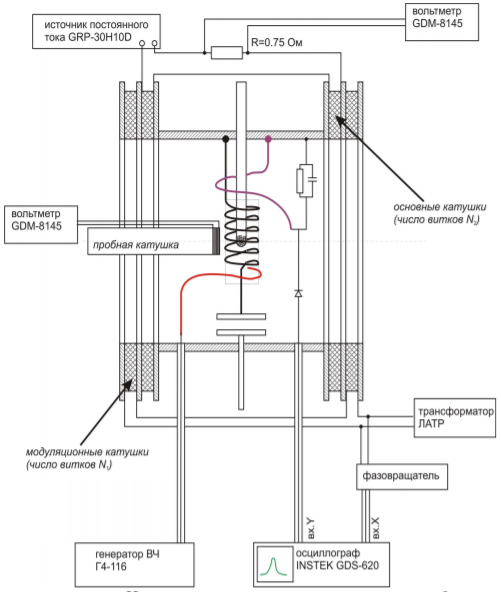
\includegraphics[width = 0.4\textwidth]{ust.png}
\centering
\caption{Схема установки.}
\end{wrapfigure}

Схема установки представлена на Рис. 1. Образец (порошок ДФПГ) в стеклянной ампуле помещается внутрь катушки индуктивности, входящей в состав колебательного контура. Входящий в состав контура конденсатор состоит из двух пластин, разделённых воздушным зазором, одна из пластин может перемещаться поворотом штока. Колебания в контуре возбуждаются антенной, соединённой с генератором высокой частоты (ВЧ) Г4-116. Амплитуда колебаний поля в катушке индуктивности
измеряется по наводимой в петле связи ЭДС индукции. Высокочастотные колебания ЭДС
индукции в приёмном контуре детектируются диодом, измеряемая при помощи
осциллографа низкочастотная огибающая этого сигнала пропорциональна квадрату
амплитуды колебаний поля в катушке.\\
Постоянное магнитное поле создаётся пропусканием тока от источника постоянного тока через основные катушки. При этом при помощи вольтметра измеряется падение напряжения на резисторе в цепи основных катушек. Переменное поле небольшой амплитуды создаётся подачей на модуляционные катушки напряжения с регулируемого трансформатора ЛАТР. Для измерения амплитуды колебаний переменного поля используется пробная катушка известной геометрии, подключённая к вольтметру. Пусть поток через неё $\Phi_{\text{проб}}$, тогда ЭДС индукции
\[\mathcal{E} = - \dfrac{d\Phi_{\text{проб}}}{dt}.\]
Если $I_{\text{осн}}$ -- ток через основную катушку, а $M$ -- взаимная индуктивность основной и пробной катушек, то
\[\Phi_{\text{проб}} = M I_{\text{осн}}.\]
Тогда амплитудное значение ЭДС индукции
\[\mathcal{E}_{\text{амп}} = - \dfrac{dM I_{\text{осн}}}{dt} = M \omega I_{\text{амп}}.\]
Учитывая, что $I_{\text{амп}} = \sqrt{2} I_{\text{действ}}=\frac{V_r}{r}$, где $V_R$, $R$ -- напряжение на резисторе с сопротивлением $R$ в цепи основных катушек, а также $\mathcal{E}_{\text{амп}} = \sqrt{2}\mathcal{E}_{\text{ср}}$, получим
\[\mathcal{E}_{\text{ср}} = M \omega \dfrac{V_R}{R} = k V_R.\]
Тогда, зная, что
\[\Phi_{\text{проб}} = B_0 N_{\text{проб}} \dfrac{\pi d_{\text{проб}}^2}{4} =  \dfrac{MU_R}{R} = \dfrac{k U}{\omega},\]
где $U$ -- напряжение на $R$ в резонансе, получим
\begin{equation}\label{1}
B_0 = \dfrac{4k U}{\pi \omega d^2_{\text{проб}} N_{\text{проб}}}.
\end{equation}

\section{Результаты измерений и обработка данных}

        \subsection*{Резонанс}
	    
	    
		Настроим генератор на частоту колебательного контура. Получаем резонансную частоту:
		\begin{equation*}
			f_0 = (162 \pm 1) \ \text{МГц}.
		\end{equation*}
	
		Подберем величину постоянного магнитного поля в катушках так, чтобы наблюдался сигнал резонансного поглощения. Для этого подадим на катушки достаточное напряжение.
		
		Для более точной настройки и определения ширины линии резонансного поглощения будем наблюдать сигнал в $XY$-режиме. 
		
		\subsection*{Определение модулирующего поля с помощью пробной катушки}
		
		Измерение индукции поля производится с помощью пробной катушки и милливольтметра. Запишем показания вольтметра в режиме измерения постоянного тока и переключим катушки на переменный ток. Для этого нужно включить вилку питания катушек в клеммы автотрансформатора и подобрать положение движков трансформатор так, чтобы показание вольтметра в режиме измерения переменного тока совпадало с записанным ранее значением. Введём пробную катушку внутрь основных катушек поблизости от образца. Измерим показания милливольтметра $V = 14~мВ$. Величину магнитного поля $B_0$ определим из формулы
$$ V = n B_0 S \omega_{\simeq},$$
где $\omega_{\simeq}$ --- угловая частота переменного тока. Характеристики пробной катушки: $n_{\text{проб}} = 44$, $d_{\text{проб}} = 14,9\pm 0,1~\text{мм}$.
 
Полученное значение $B_0 = 5,81\pm0,12~мТл$.

		\subsection*{Расчёт g-фактора электрона}
		
		Найдем $g$-фактор электрона:
		
		\begin{equation*}
			g = \frac{hf_0}{\mu_BB_0} = 2,02 \pm 0,04.
		\end{equation*}

		\subsection*{Ширина линии поглощения}
	
		Определим ширину линии ЭПР (полуширина на полувысоте линии резонансного поглощения):
		\begin{equation*}
			\Delta B = \frac{A_{1/2}}{A_{\text{полн}}}B_\text{мод},
		\end{equation*}
		где $A_\text{полн}$ --- полный размах модулирующего поля, $A_{1/2}$ --- ширина кривой на полувысоте, $B_\text{мод}$ --- амплитуда модулирующего поля.
		\begin{equation*}
			\begin{gathered}
				A_\text{полн} = 3 \ \text{дел}, \ A_{1/2} = 1 \ \text{дел} \\
				B_\text{мод} = 5,81\pm0,12~мТл.
			\end{gathered}
		\end{equation*}
		
		Имеем:
		\[\boxed{\Delta B = (1,94 \pm 0,04) \ \text{мТл}}.\]
		
\section{Обсуждение результатов и выводы}

В данной работе был исследован ЭПР в молекуле ДФПГ, определяется $g$-фактор электрона $g = 2,02 \pm 0,04$, а также измерена ширина линий ЭПР $\Delta B = 1,94 \pm 0,04~\text{мТл}$.

	Измеренный $g$-фактор электрона совпадает с табличным значением для свободного электрона: $g = 2,0$. Это обусловлено тем, что ПР происходит на неспаренных электронах так же, как на свободных.
\end{document}
